\chapter{Deterministic Models}

\section{Linear Programming}

The best way to learn the art of mathematical modeling is through practice.
We begin with a simple two-variable Linear Programming model whose solution
will inform the owner of a business how to allocate scarce resources to achieve
maximum profit. Additional information returned with the solution will be used
to gain insight on obtaining additional resources and an idea of the robustness
of the solution to small changes in the data.
Along the way we will
illustrate various features of the GAMS algebraic modeling language. 
\footnote{We do not provide a complete introduction to GAMS.
Excellent tutorials already exist. \cite{Rosenthal,GAMS}.}

Why use GAMS? Well, it's not GAMS in particular, but rather
algebraic modeling languages in general that are extremely useful
when \emph{formulating} mathematical programming problems
\footnote{AMPL is another popular algebraic modeling language with a 
clear and expressive syntax \cite{fourer:2003}.} An
algebraic modeling language allows one to easily specify and
understand objective functions, constraints, and logical relationships
among variables. The syntax of the GAMS language is simple,
yet expressive enough to enable many different types of problems to be
directly modeled. We should note that GAMS is not a general-purpose
programming language, although it does contain constructs for
conditional execution of statements and for iterative looping.
Rather, GAMS is an example of a \emph{domain-specific} language.  Its
purpose is to facilitate translation from a problem description into a
form that is suitable for a solver to process.

\emph{A resource allocation problem.}
A local farmer maintains 500 acres on which she can grow feed corn for animals
and/or organic corn for local millers. As the planting season approaches,
she must decide how many acres to allocate to each type of corn.
Her operating budget is \$\num{50000}. The costs and returns for each
type of corn are as follows.

\vspace{.1in}
\begin{tabular}{rrr}
type & cost per acre & revenue per acre \\ \hline
feed corn & \$90 & \$200 \\
organic corn & \$150 & \$300
\end{tabular}
\vspace{.1in}

A natural objective is to maximize total profit, and organic appears to be 
more attractive; however, the farmer must
respect both her operating budget and the available acres. If we let $x1$ and 
$x_2$ represent the 
number of acres to allocate to feed corn and organic corn, respectively,
then the farmer's decision problem is to
\[
\begin{array}{lrrrrrl}
\textrm{maximize}   & 110x_1 & + & 150x_2 & = &  & z \textrm{(profit)} \\
\textrm{subject to} & 90x_1 & + & 150x_2 & \leq & \num{50000} & \textrm{(budget)} \\
                    & x_1 & + & x_2   & \leq & 500  & \textrm{(acres)} \\
\multicolumn{4}{r}{x_1,x_2}& \geq & 0 &
\end{array}.
\]

The operating budget and the available acres are constrained resources in
the sense that if the farmer could obtain a little more of either resource,
then she could earn more profit. Later in the section, will make this 
notion more precise. Since this problem has two decision variables, the 
inequalities that describe the constraints can be shown graphically
as in Figure~\ref{fig:feasibleregion}. Any combination of $x_1$ (feed corn)
and $x_2$ (organic corn) within the shaded area represents a feasible
solution for the farmer. The optimal solution is the combination that 
maximizes total profit.

The constraints in Figure~\ref{fig:feasibleregion} were drawn by 
\begin{inparaenum}[1)]
\item representing the inequality as a line, and then 
\item determining on which side of line the inequality is valid. 
\end{inparaenum}
The dashed line represents the objective function, but it is drawn at an
arbitrary place in the figure. The important thing to note is the
slope. Writing the objective as
\[ x_2 = \frac{z}{150} - \frac{110}{150}x_1 \]
lets us easily see that the slope is $-11/15$. Now, to find the
values of the decision variables ($x_1$ and $x_2$) that maximize
the expression
\[ z = 110x_1 + 150x_2 \]
while still satisfying the constraints, imagine sliding the dashed line
up and to right until the point just before the dashed line leaves the
feasible region. This will occur at the point where the two 
lines representing the constraints intersect, i.e. $x_1 = 416.67$, $x_2 = 83.33$.
The optimal solution to any linear programming problem will always
occur at a "corner point". We can determine which corner point by comparing
the slope of the objective function to the slopes of the lines representing the
constraints that define the feasible region. In this case the slope of the objective
function $-11/15$ is "steeper" that the slope of the budget constraint $=9/11$, but
not as steep as the slope of the acres constraint $-1$. Typically, a
linear programming problem will have many variables and constraints, but the same
ideas apply. Indeed, the kernel of the idea behind the Simplex algorithm,
the workhorse algorithm that is commonly used to solve linear programming problems, 
is to move from corner
point to corner point, each time increasing the value of the objective
function until no further improvements can be made.

\begin{figure}
\begin{center}
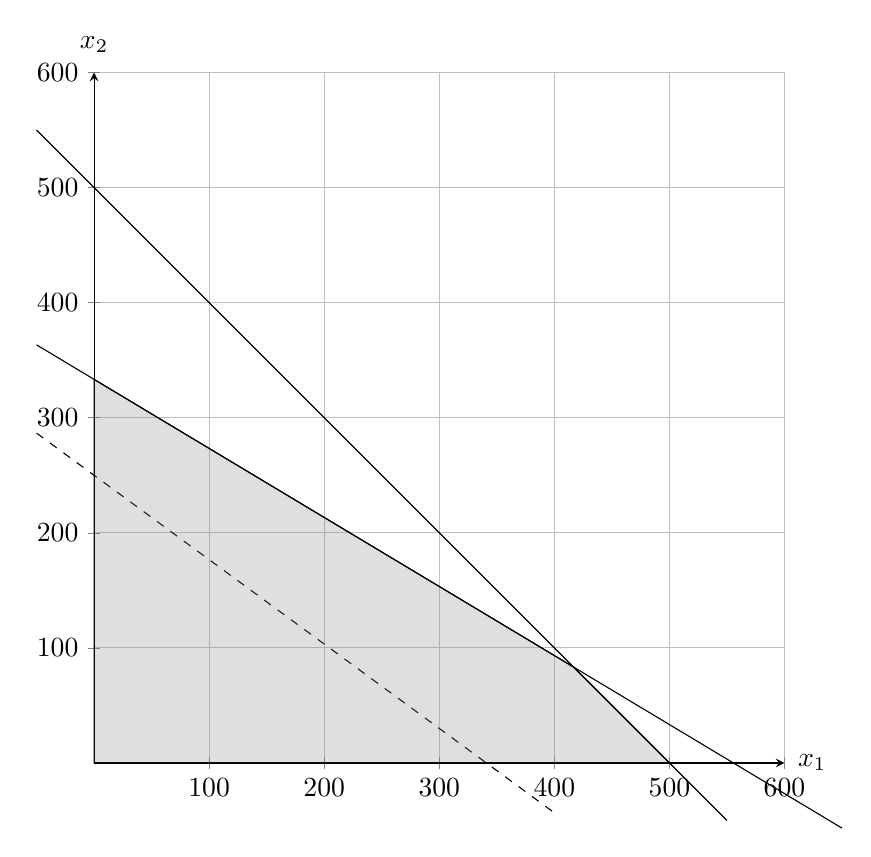
\begin{tikzpicture}
  \begin{axis}[ width=12cm,
    unit vector ratio*=1 1 1,
    enlargelimits=false,
    grid=both,
    axis x line=middle,
    axis y line=middle,
    title=,
    clip=false,
    ymin=0, ymax=600,
    xmin=0, xmax=600]

    \addplot[domain=-50:650] {50000/150 - 90/150*x};
    \addplot[domain=-50:550] {500 - x};
    \addplot[domain=-50:400,dashed] {250 - 110/150*x};
    \addplot[fill=gray, fill opacity=.25]
    coordinates { (0,0) (500,0) (416.67,83.33) (0,333.33) } \closedcycle;

  % to get axis labels at the end of the axis
  \node at (axis description cs:1.04,0) {$x_1$}; \node at
  (axis description cs:0,1.04) {$x_2$};
\end{axis}
\end{tikzpicture}
\end{center}
\caption{Feasible region for the farm problem.}
\label{fig:feasibleregion}
\end{figure}

We now show how to model the farm problem in GAMS.
The complete problem formulation is shown in
figure~\ref{fig:farmer}.

\begin{SaveVerbatim}{vrbfarmer}
variables
x1 'acres of feed corn'
x2 'acres of organic corn'
z;
positive variables x1, x2;

equations
 profit  'objective function'
 budget  'available cash'
 acres   'available acres';

profit.. z =e= 110*x1 + 150*x2;
budget.. 90*x1 + 150*x2 =l= 50000;
acres.. x1 + x2 =l= 500;

model farmer / all /;

solve farmer using LP maximizing z;
\end{SaveVerbatim}

\begin{figure}
\fbox{
\begin{minipage}{\textwidth}
\BUseVerbatim{vrbfarmer}
\caption{Farm problem (\texttt{farmer.gms})}
\label{fig:farmer}
\end{minipage}
}
\end{figure}


Since this problem is small, we include all data parameters directly
in the model specification. However, it is usually good practice to
separate the data from the model, and AMPL encourages this separation
by providing \texttt{param} declarations and the ability to have a
separate \texttt{data} section. We will illustrate these features of
AMPL in the other problem formulations in this article.  AMPL doesn't
actually solve the mathematical programing problem, but rather passes
a description of the problem to a solver, which returns information
about the solution (if any solution was found) to AMPL. An AMPL
session for the forestry problem follows:

\begin{Verbatim}[samepage=true]
ampl: model forester.mod;
ampl: solve;
MINOS 5.5: optimal solution found.
2 iterations, objective 6250
ampl: display x1,x2;
x1 = 25
x2 = 75
\end{Verbatim}

The optimal solution indicates that the forester should harvest 100
acres, but let 25 acres regenerate naturally and plant 75 acres with
pine, for a profit of \$6250. Notice that the entire budget of \$4000
is exhausted because $10 \times 25 + 50 \times 75 = 4000$. When a
resource capacity constraint such as \texttt{acres} or \texttt{budget}
holds with equality in the optimal solution (as in this example), then
the constraint is \emph{binding}; all of the resource associated with
the constraint is being consumed. If more/less of the resource were
available, then profit would be increased/decreased. The value of the
associated dual variable indicates the amount by which profit would be
affected for small changes in the supply of the resource. This is
called the marginal value of a resource, or the shadow price.

\begin{Verbatim}[samepage=true]
ampl: display acres, budget;
acres = 32.5
budget = 0.75
\end{Verbatim}

Displaying the shadow prices in AMPL indicates that an additional acre
of hardwood timber would increase profit by \$32.50, given the same
budget of \$4000.  Modifying the right-hand side of \texttt{acres} to
101 and re-solving shows that this is indeed the case.

\begin{Verbatim}[samepage=true]
ampl: reset;
ampl: model forester.mod;
ampl: expand acres;
subject to acres:
	x1 + x2 <= 101;

ampl: solve;
MINOS 5.5: optimal solution found.
2 iterations, objective 6282.5
ampl: display x1,x2;
x1 = 26.25
x2 = 74.75
\end{Verbatim}

The \texttt{expand} command displays the full form of a set of
constraints.  (This will be useful for indexed expressions.) Notice
that the values of the decision variables have necessarily changed and
that the solution is no longer integer-valued.  This is typical of
resource allocation problems. We are in fact assuming that the
forester is able to execute the decisions on partial acres.  For the
\texttt{budget} constraint, an additional one dollar increase/decrease
in the right-hand side would increase/decrease profit by \$0.75, given
the same 100 acres of hardwood. It stands to reason, then, that the
forester could take out a loan and apply the funds to her
operation. As long as the interest rate is less than .75, profit will
increase.

Shadow prices are valid for \emph{limited} increases/decreases in the
right-hand sides of the constraints. The ranges over which the these
values are valid is a topic of sensitivity analysis. Here, we will
show how to extract this information from AMPL. First we need to tell
AMPL to use a solver that is able to return sensitivity information
along with the optimal solution. We will use the solver
\texttt{cplex}. Then we set a solver-specific option to make the
sensitivity range information available.

\begin{Verbatim}[samepage=true]
ampl: option solver cplex;
ampl: option cplex_options 'sensitivity';
ampl: solve;
CPLEX 11.2.0: sensitivity
CPLEX 11.2.0: optimal solution; objective 6250
2 dual simplex iterations (1 in phase I)

suffix up OUT;
suffix down OUT;
suffix current OUT;
\end{Verbatim}

We are now able to display the ranges over which the current shadow
prices of \$32.5 per acre and \$0.75 per dollar of budget are
valid. To do this we simply add a suffix to the name of the
constraint, separated by a ``\texttt{.}''. The suffix
\texttt{.current} displays the current value of a constraint's
right-hand side, while \texttt{.down} and \texttt{.up} display the
lower and upper limits, respectively. In the AMPL session follows, the
upper limit of 5000 on the right-hand side of \texttt{budget}
indicates the forester should only consider loans of \$1000 or less to
be valued at an incremental marginal value of 0.75.

\begin{Verbatim}[samepage=true]
ampl: display acres.down, acres.current, acres.up;
acres.down = 80
acres.current = 100
acres.up = 400

ampl: display budget.down, budget.current, budget.up;
budget.down = 1000
budget.current = 4000
budget.up = 5000
\end{Verbatim}

Sensitivity ranges may also be obtained for the decision variables. In
this case the lower and upper limits represent the valid ranges on the
objective function coefficients over which the current solution
remains optimal.  The suffix \texttt{.current} refers to the current
value of the coefficient.  Displaying this information for the
forestry problem reveals that the current solution value of \texttt{x1
  = 25} remains optimal as long as its coefficient in the objective
function is in the range 14 to 70, holding all other parameters at
their current values.

\begin{Verbatim}[samepage=true]
ampl: display x1.down, x1.current, x1.up;
x1.down = 14
x1.current = 40
x1.up = 70

ampl: display x2.down, x2.current, x2.up;
x2.down = 40
x2.current = 70
x2.up = 200
\end{Verbatim}

\emph{A Diet Problem.}
Dwight is an elementary school teacher who also raises pigs for
supplemental income. He is trying to decide what to feed his pigs.
Considering a combination of pig feeds available from local suppliers,
he would like to feed the pigs at minimum cost while also making sure
each pig receives an adequate supply of calories and vitamins.  The
cost, calorie content, and vitamin content of each feed are given in
the table below.

\vspace{.1in}
\begin{center}
\begin{tabular}{ccc}
\textbf{Contents}   &  \textbf{Stark County Coop Pig Feed }   & \textbf{Pioneer Pig Feed} \\   \hline
Calories (per pound)  &  800    &  1000   \\
Vitamins (per pound)  &  140 units  &  70 units  \\
Cost (per pound)   &  \$0.40    & \$0.80  \\
\end{tabular}
\end{center}
\vspace{.1in}

Each pig requires at least 8,000 calories per day and at least 700
units of vitamins. A further constraint is that no more than one-third
of the diet (by weight) can consist of Stark County Coop Pig Feed,
since it contains an ingredient which is toxic if consumed in too
large a quantity.  First, let's write down the mathematical
programming formulation without regard to AMPL. Let $x_1$ be the
pounds per day of Stark County Coop feed to purchase. Similarly, let
$x_2$ be the pounds per day of Pioneer feed to purchase. Then the
problem is to 

\[
\begin{array}{lrrrrrl}
\textrm{minimize}   & .4x_1 & + & .8x_2 &  &  &  \\
\textrm{subject to} & 800x_1 & + & 1000x_2 & \geq & 8000 & \textrm{(calories)} \\
                    & 140x_1 & + & 70x_2   & \geq & 700  & \textrm{(vitamins)} \\
					& 2x_1   & - & x_2     & \leq & 0    & \textrm{(toxicity)} \\
\multicolumn{4}{r}{x_1,x_2}& \geq & 0 &
\end{array}.
\]

To get the toxicity restriction on the amount of Stark County Coop
feed, begin with the relation
\[
x_1 \leq \frac{1}{3}(x_1 + x_2).
\]
Then collect terms and simplify.  Since this problem has only two
variables, we can easily specify the model in AMPL by creating each
variable, the objective function, and the three constraints as shown
in Figure~\ref{p1}. This model should be saved in a text file with a
\texttt{.mod} extension.

\begin{SaveVerbatim}{pigs}
var x1 >= 0;  # stark
var x2 >= 0;  # pioneer

minimize total_cost: .4*x1 + .8*x2;

subject to cal: 800*x1 + 1000*x2 >= 8000;
subject to vit: 140*x1 + 70*x2 >= 700;
subject to tox: x1 <= (1/3)*(x1 + x2);
\end{SaveVerbatim}

\begin{figure}
\fbox{
\begin{minipage}{\textwidth}
\BUseVerbatim{pigs}
\caption{AMPL model (\texttt{pigs.mod})}
\label{p1}
\end{minipage}
}
\end{figure}

The following AMPL session shows how to read the problem into AMPL,
invoke the default solver, and print the solution. The minimum cost
feed mixture is 2.86 pounds of Stark County feed and 5.71 pounds of
Pioneer feed per pig per day, for a total cost of \$5.71 per pig per
day.
\begin{Verbatim}[samepage=true]
ampl: model pigs.mod;
ampl: solve;
MINOS 5.51: optimal solution found.
2 iterations, objective 5.714285714
ampl: display x1, x2;
x1 = 2.85714
x2 = 5.71429
\end{Verbatim}

For problems of any reasonable size it is necessary (and desirable) to separate
the model and data. This will allow us to solve different problem instances
(i.e. different sets of data) without changing the model. Figure~\ref{p2} shows
the complete problem formulation and data with separate \texttt{model} and
\texttt{data} sections in the same text file (\texttt{pigs2.mod}). It is also
possible (and you will usually want to do this) to put the data section
in its own text file. In that case we would name the data file with a
\texttt{.dat} extension, e.g. \texttt{pigs2.dat}.

\begin{SaveVerbatim}{pigs2}
model;
set Supplier;

param calories {Supplier};  # per pound
param vitamins {Supplier};  # units per pound
param cost {Supplier};      # dollars per pound

var x {Supplier} >= 0;  # pounds to purchase from each supplier (per pig)

minimize total_cost: sum {i in Supplier} cost[i]*x[i];

s.t. cal: sum {i in Supplier} calories[i]*x[i] >= 8000;
s.t. vit: sum {i in Supplier} vitamins[i]*x[i] >= 700;
s.t. tox: x['stark'] <= (1/3)* sum {i in Supplier} x[i];

data;
set Supplier := stark pioneer;

param : vitamins cost calories:=
stark   140      .4    800
pioneer  70      .8   1000;
\end{SaveVerbatim}

\begin{figure}
\fbox{
\begin{minipage}{\textwidth}
\BUseVerbatim{pigs2}
\caption{Separation of model and data (\texttt{pigs2.mod})}
\label{p2}
\end{minipage}
}
\end{figure}

Most AMPL models are specified by declaring sets, parameters, and
variables, and then by writing the objective function and the
constraints that make use of the sets, parameters, and
variables. Parameters are typically numeric values, although they can
also be logical or symbolic values. They can be thought of as ``data''
values, e.g. the cost per pound of feed. Variables represent the
decisions, e.g. the amount of feed to purchase. Sets specify the
objects with which parameters and variables are associated. We
declared the feed suppliers to be a set because the decisions for how
much feed to purchase as well as cost and nutritional attributes of
the feed are logically associated with each supplier. We say that the
parameters and the variables are \emph{indexed} over the set of
suppliers.

Giving short, meaningful names to sets, parameters, and variables
makes a model readable.  I like to capitalize the first letter of set
names so that they are easily distinguished from parameters.  In the
AMPL book, you will see that set names are in all upper-case
letters. This is just a convention, and the language does not require
it; however, good programming habits will make your code easier to
maintain.

Here is the output from an AMPL session using the model and data in
\texttt{pigs2.mod}.  When working with AMPL, if you read in a model
and subsequently make changes, or if you read in a new model after
having worked with an initial model, you will need to use the
\texttt{reset} command before reading in the new model. Note that when
the decision variables are indexed over a set, we display all of them
at once by typing the variable symbol.
\begin{Verbatim}[samepage=true]
ampl: reset;
ampl: include pigs2.mod;
ampl: solve;
MINOS 5.51: optimal solution found.
2 iterations, objective 5.714285714
ampl: display x;
x [*] :=
pioneer  5.71429
  stark  2.85714
;
\end{Verbatim}

\emph{Factory Planning.}
This example is taken from~\cite{williams:1999}. 
A factory makes seven products that require various amounts of time on four different
types of machines. The factory owns four grinders, two vertical drills, three 
horizontal drills, one boring machine, and one planing machine. 
For each product manufactured, the company can either sell the
product (subject to market limitations) or hold the product in inventory at a cost of
.5 per unit per month. We would like to develop a production and inventory plan for
each of the next six months.
We will not consider the sequence of machine operations; however, there
is a fixed maintenance schedule that specifies when and how many of each machine type
will be unavailable. The factory operates two eight-hour shifts each working day.
There are 24 working days each month.

Refer to the data in figure~\ref{fdat} as well as the model in
figure~\ref{fmod} while reading this description.
Notice that the set \texttt{Month} is declared to be of type \texttt{ordered},
indicating a defined ordering among its (symbolic) members.
This means that we can refer to the members of \texttt{Month} by their relative position.
For example, in our data the expression \texttt{first(Month)} refers
to the member \texttt{'jan'}. One common reason for declaring a set to be \texttt{ordered}
is the need to refer to the previous and/or the next member in an indexed expression.
A typical example of this use of an \texttt{ordered} set is illustrated by the 
\texttt{balance} constraints.

\begin{SaveVerbatim}{vrbfmod}
set Product;
set Machine;
set Month ordered;

param profit {Product} >= 0;
param time_required {Product,Machine} >= 0;
param num_available {Machine} integer, >= 0;
param downtime {Month,Machine} integer, >=0;
param market_limit {Month,Product} integer, >= 0;
param work_hours := 2*8*24;
# number of working hours in a month: 2 shifts of 8 hours each, 24 days/month

var make {Month,Product} >=0;  # how much of each product to make in each month
var sell {Month,Product} >=0;  # how much to sell
var hold {Month,Product} >=0, <=100;  # how much to hold

maximize total_profit:
  sum {t in Month, i in Product} (profit[i]*sell[t,i] - 0.5*hold[t,i]);

s.t. capacity {t in Month, m in Machine}:
sum {i in Product} time_required[i,m]*make[t,i] 
  <= work_hours*(num_available[m]-downtime[t,m]);

s.t. marketing {t in Month, i in Product}: sell[t,i] <= market_limit[t,i];

s.t. balance {t in Month, i in Product : ord(t) > 1}:
  hold[prev(t),i] + make[t,i] = sell[t,i] + hold[t,i];
# on-hand inventory plus number produced must equal number
# sold plus number held in inventory for the next period

s.t. balance0 {i in Product}:
  make[first(Month),i] = sell[first(Month),i] + hold[first(Month),i];
# there is no inventory held over from december

s.t. end_inventory {i in Product}: hold[last(Month),i] = 50;
# stipulate that 50 of each product are to be held over from june
\end{SaveVerbatim}

\begin{figure}
\fbox{
\begin{minipage}{\textwidth}
\BUseVerbatim{vrbfmod}
\caption{Model for factory planning problem (\texttt{factory\_planning1.mod})}
\label{fmod}
\end{minipage}
}
\end{figure}

A defining feature of this model is use of three different variables to represent
the quantities and timing for making, selling, and holding each product.
The relationship among these
variables is stated in the \texttt{balance} constraints.
An upper bound of 100 units on the \texttt{hold} variable represents a storage limitation 
for each product in each month.

Our objective is to maximize the total profit of the factory over a period of six months.
A unit profit is accrued for each item sold and a unit cost of .5 is incurred for each item
held in inventory in a given month.
Note that the parentheses surrounding the subtraction
are necessary because the \texttt{sum} operator has higher precedence than \texttt{-}.
As a side note, if we were to remove the holding cost from consideration in 
the objective then no parentheses would be required around the
\texttt{profit[i]*sell[t,i]} term because the \texttt{sum} operator has lower precedence
than \texttt{*}~\cite{fourer:2003}. 

Each product requires a certain amount of processing time (possibly zero) on each type
of machine. These requirements are specified in the data by the parameter 
\texttt{time\_required} that is indexed over \texttt{Product} and \texttt{Machine}
We need to specify constraints on the amount of machine time
available each month. There are \texttt{work\_hours} production hours available each month
on each machine unless a machine is down for maintenance. Because the maintenance
schedule is specific to each machine and month, the machine capacity constraints 
are indexed over \texttt{Month} and \texttt{Machine}. The total number of machine
hours for all products must not exceed the time available in any particular month
(respecting the \texttt{downtime} schedule.)
There is an upper bound on the amount of each product that the market will absorb
(i.e. that can be sold) each month.

We have three different variables to represent the decisions to make, sell,
and hold product.  The logical relationship among these variables is that
in any particular month the amount sold plus the amount held in inventory
must equal the amount produced plus any inventory from the previous month.
When specifying these product balance constraints we must pay attention to the
boundary conditions when indexing over \texttt{Month}. In our problem, we
cannot refer to the previous month when the dummy index evaluates to \texttt{'jan'}.
We can handle this in the main \texttt{balance} equations by placing a condition
on the indexed set such that the order of the member is greater than 1
(and so \texttt{'jan'} is omitted.)
This is possible because we declared the set \texttt{Month} to be of type
\texttt{ordered}. We then need to specify a separate set of constraints for
the first month (\texttt{balance0}). There is no beginning inventory and 
so the amount produced in \texttt{'jan'} equals the amount sold plus the amount
held.

Instead of using the expression \texttt{make[first(Month),i]},
it would have been legitimate to refer to \texttt{make['jan',i]}; however,
it's better practice to separate the model from the data. The model may then
be applied to other problem instances with the same structure, but perhaps with
a different starting month. Finally, we would like to end June with 50 of
each product type in inventory. This is specified by the equality constraints
named \texttt{end\_inventory}.

\begin{SaveVerbatim}{vrbfdata}
data;
set Product := 1 2 3 4 5 6 7;
set Machine := grinder vdrill hdrill borer planer;
set Month := jan feb mar apr may jun;

param profit := 1 10 2 6 3 8 4 4 5 11 6 9 7 3;

param num_available :=	
grinder 4 vdrill 2 hdrill 3 borer 1 planer 1;

param time_required (tr) :
         1   2   3   4   5   6   7 :=
grinder .5  .7   0   0  .3  .2  .5
vdrill  .1  .2   0  .3   0  .6   0
hdrill  .2   0  .8   0   0   0  .6
borer  .05 .03   0 .07  .1   0 .08
planer   0   0 .01   0 .05   0 .05;

param downtime :
     grinder vdrill hdrill borer planer :=
jan    1       0     0      0     0
feb    0       0     2      0     0
mar    0       0     0      1     0
apr    0       1     0      0     0
may    1       1     0      0     0
jun    0       0     1      0     1;

param market_limit :
       1     2     3     4     5     6     7 :=
jan  500  1000   300   300   800   200   100
feb  600   500   200     0   400   300   150
mar  300   600     0     0   500   400   100
apr  200   300   400   500   200     0   100
may    0   100   500   100  1000   300     0
jun  500   500   100   300  1100   500    60;
\end{SaveVerbatim}

\begin{figure}
\fbox{
\begin{minipage}{\textwidth}
\BUseVerbatim{vrbfdata}
\caption{Data for factory planning problem (\texttt{factory\_planning1.mod})}
\label{fdat}
\end{minipage}
}
\end{figure}

\section{Integer Programming}

\emph{Perfect Matching.}
There are 10 students to be assigned to 5 dorm rooms. Each room holds exactly
two students. For each pair of students, a value that indicates the desirability
of placing that pair in the same room has been determined. Higher values 
correspond to better pairings.
We would like to pair the students in such a way that the
sum total of the values of each assigned pair is maximized. More generally,
the perfect matching problem is to assign $n$ pairs for $2n$ objects (with or without
an objective function). The model and data are presented in figure~\ref{perfect}.

\begin{SaveVerbatim}{vrbperfect}
set Student; 
set Pair within Student cross Student;

param value {Pair};

var x {Pair} binary;

maximize total_value: sum {(i,j) in Pair} value[i,j] * x[i,j];

s.t. perfect_match {i in Student}:
	sum {(i,j) in Pair} x[i,j] + sum {(j,i) in Pair} x[j,i] = 1;

data;
set Student := 1 2 3 4 5 6 7 8 9 10;

param: Pair: value:
   1  2  3  4  5  6  7  8  9 10 :=
1  .  .  .  .  .  .  .  .  .  .
2  3  .  .  .  .  .  .  .  .  .
3  5  8  .  .  .  .  .  .  .  .
4  1 -4  7  .  .  .  .  .  .  .
5  2 -1  9  2  .  .  .  .  .  .
6  2  5  3  2  9  .  .  .  .  .
7  8  2  1  1  3 -2  .  .  .  .
8  2  3  3  4  5  1  1  .  .  .
9 13 -1  3  4  4 -5  2  2  .  .
10 1  2  6  6  7 -4  5  6  1  .;
\end{SaveVerbatim}

\begin{figure}
\fbox{
\begin{minipage}{\textwidth}
\BUseVerbatim{vrbperfect}
\caption{Model and data for perfect matching problem (\texttt{roommates.mod})}
\label{perfect}
\end{minipage}
}
\end{figure}

\texttt{Pair} is a compound set with dimension two. Each member of this set is
an ordered pair of students. We use the term ``ordered'' because the member
(3,7) is distinct from the member (7,3). The \texttt{within} phrase tells
us that the only allowed members in \texttt{Pair} are ordered pairs from the set
\texttt{Student}. Such restrictions in the declaration of sets are encouraged in order to
help detect errors in the data. For example, the following alternative declaration is 
perfectly acceptable, but using it would not allow the AMPL translator to recognize
invalid pairs of students in the data section.
\begin{Verbatim}
set Pair dimen 2;
\end{Verbatim}

The declaration of \texttt{Pair} is not strictly necessary. We could formulate the problem
using only the set \texttt{Student}. However, using the compound set \texttt{Pair}
makes the model easier to read and to maintain, particularly the indexing expressions.
We specify a parameter \texttt{value} that is indexed over \texttt{Pair} to represent the
desirability of matching up a particular pair of students. Our decision variables
\texttt{x} are binary variables that are also indexed over \texttt{Pair}. 
\texttt{x[i,j]} will equal one if student \texttt{i} is matched with student \texttt{j},
and will equal zero otherwise. Notice the \texttt{binary} modifier in the declaration
of \texttt{x}. This means that our decision variables may \emph{only} take on the values zero
or one and turns our formulation into one of pure integer programming~\cite{nemhauser:1988}.

The problem formulation itself consists of the objective function and a single set
of constraints, one for each student. Our objective is to maximize the overall
value of the assignments. It provides a good example of how to iterate over a 
compound set in AMPL. Notice that we must provide a pair of dummy variables
\texttt{(i,j)} to index into \texttt{Pair}. 

The constraints \texttt{perfect\_match} state that each student must be
matched with exactly one other student. To understand how this is 
accomplished note that the scope of the index \texttt{i} extends from 
its introduction in \texttt{i in Student} until the end of the statement
marked by the semi-colon. In the expression \texttt{sum \{(i,j) in Pair\} x[i,j]},
\texttt{i} is held constant for a particular student (row of \texttt{value}) 
and the summation is over all room mates such that the pair of students
represented by \texttt{(i,j)} exist in the set \texttt{Pair}, i.e. the
summation is over columns.
In the second expression with \texttt{i} and \texttt{j} interchanged, the
summation is over rows. This is necessary
due to the way that the data for \texttt{Pair} are structured. Notice that
only the lower left portion of \texttt{value} is filled in.

This example demonstrates how to simultaneously define a set (\texttt{Pair}) and a parameter
(\texttt{value}) that is indexed over that set. The ``\texttt{.}'' symbols indicate
missing values, e.g. there exists no member \texttt{(1,1)} in the set \texttt{Pair}.
An AMPL session for solving this problem follows. Although not strictly necessary
for this particular problem, we will instruct AMPL to use
a solver that can handle integer programming problems, such as the solver
\texttt{gurobi}. 

\begin{Verbatim}[samepage=true]
ampl: option solver gurobi;
ampl: model roommates.mod;
ampl: solve;
Gurobi 3.0.0: optimal solution; objective 39
14 simplex iterations
ampl: display x;
x [*,*]
:    1   2   3   4   5   6   7   8   9    :=
2    0   .   .   .   .   .   .   .   .
3    0   1   .   .   .   .   .   .   .
4    0   0   0   .   .   .   .   .   .
5    0   0   0   0   .   .   .   .   .
6    0   0   0   0   1   .   .   .   .
7    0   0   0   0   0   0   .   .   .
8    0   0   0   1   0   0   0   .   .
9    1   0   0   0   0   0   0   0   .
10   0   0   0   0   0   0   1   0   0
;
\end{Verbatim}

The large number of zeros makes the solution difficult to read. A useful
option is to only display the decision variables with nonzero values. Then
we can easily see that the pairs are (3,2),(6,5),(8,4),(9,1), and (10,7).

\begin{Verbatim}[samepage=true]
ampl: option omit_zero_rows 1;
ampl: display x;
x :=
3  2   1
6  5   1
8  4   1
9  1   1
10 7   1
;
\end{Verbatim}

\emph{Map Coloring.}
The map coloring problem is to assign a color to each area on a map
(e.g. state or county) in such a way that adjacent areas (i.e. those
areas that share a border) are assigned different colors. Moreover, we 
would like to use as few colors as possible. The formulation for this
problem was adapted from code written in GNU MathProg by Andrew
Makhorin~\cite{glpk}.

We may create a representation of the adjacency information by constructing a
graph wherein each area on the map is represented by a node. An 
edge is drawn between two nodes if the respective areas on the map share a border.
As an example, figure ? shows the map and the corresponding
adjacency graph for the western United States. The graph representation
will better facilitate the requirement that adjacent areas must be assigned 
different colors.

\begin{figure}
\begin{center}
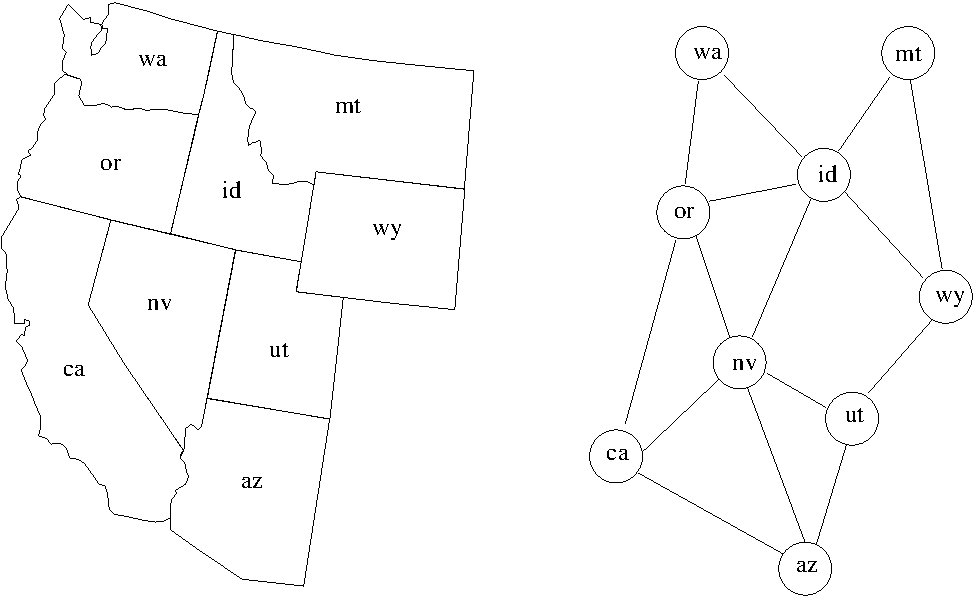
\includegraphics[scale=0.7]{westernusa.pdf}
\caption{Western states and adjacency graph}
\label{westernusa}
\end{center}
\end{figure}

Both the model and the data are presented in figure~\ref{kcolor}. In this model
we must make the cardinality of the set \texttt{Color} large enough to effect
a feasible solution. For a large problem the minimum number of colors needed will not
be obvious (otherwise there is no need to solve the problem.) However, if the 
solver finds that the problem is infeasible we can always add more members to the
set \texttt{Color}. See Andrew Makhorin's code~\cite{glpk} for an implementation
of a heuristic to obtain an upper bound on the required number of colors.

\begin{SaveVerbatim}{vrbkcolor}
set Node;
set Edge within (Node cross Node);
set Color;   
# the cardinality of the set Color needs to be large enough
# to find a feasible solution

var x {Node,Color} binary; # x[i,c] = 1 means that node i is assigned color c
var u {Color} binary;      # u[c] = 1 means that color c is used

minimize num_colors: sum {c in Color} u[c];

s.t. assignment {i in Node}: sum {c in Color} x[i,c] = 1;
# each node is assigned exactly one color

s.t. different {(i,j) in Edge, c in Color}: x[i,c] + x[j,c] <= u[c];
# adjacent nodes must be assigned different colors

data;
set Color := red blue green yellow orange;

set Node := ca or wa mt id nv wy ut az;

set Edge:
   ca or wa mt id nv wy ut az :=
ca -  +  -  -  -  +  -  -  +
or -  -  +  -  +  +  -  -  -
wa -  -  -  -  +  -  -  -  -
mt -  -  -  -  +  -  +  -  -
id -  -  -  -  -  +  +  +  -
nv -  -  -  -  -  -  -  +  +
wy -  -  -  -  -  -  -  +  -
ut -  -  -  -  -  -  -  -  +
az -  -  -  -  -  -  -  -  -;
\end{SaveVerbatim}

\begin{figure}
\fbox{
\begin{minipage}{\textwidth}
\BUseVerbatim{vrbkcolor}
\caption{Model and data for map coloring problem (\texttt{kcolor.mod})}
\label{kcolor}
\end{minipage}
}
\end{figure}

Our binary decision variables \texttt{x} will indicate the particular color 
assigned to each node (area on the map). We also create binary modeling variables
\texttt{u} to indicate that a color has been used in the solution. Now the
objective is a simple summation over \texttt{u}. There are three dummy variables
in the indexing expression for the \texttt{different} constraint. Notice
that even though \texttt{x} is indexed over \texttt{\{Node,Color\}} the
indexing expression for \texttt{different} will only create one constraint for
each existing \texttt{Edge} and \texttt{Color} combination. Since \texttt{Edge}
is declared to be \texttt{within (Node cross Node)} we may safely use the
dummy indices \texttt{i} and \texttt{j} when indexing into \texttt{x}.

In the \texttt{data} section we see one way to specify the members of a 
two-dimensional set: the ``\texttt{+}'' symbols indicate membership while the
``\texttt{-}'' symbols indicate non-membership. Alternatively, we could have
specified \texttt{Edge} by providing only the ordered pairs.
\begin{Verbatim}[samepage=true]
set Edge :=
(ca,or)   (ca,az)   (or,id)   (wa,id)   (mt,wy)   (id,wy)   (nv,ut)   (wy,ut)
(ca,nv)   (or,wa)   (or,nv)   (mt,id)   (id,nv)   (id,ut)   (nv,az)   (ut,az);
\end{Verbatim}

\section{Deterministic Dynamic Programming}

\section{Deterministic Inventory Models}

\clearpage
\section{Exercises}
\begin{enumerate}

\subsubsection*{Linear Programming}

% written by Hannah
\item \emph{Feasible region for an LP.} Indicate graphically whether each of the following
  linear programs has a feasible solution. Graphically determine the
  optimal solution, if one exists, or show that no optimal solution
  exists.

\begin{enumerate}
\item
\[
  \begin{array}{lrrrrr}
    \textrm{maximize}   & x_1& +& 3x_2&  & \\
    \textrm{subject to} & x_1& -&4x_2& \leq & 4  \\
                        & x_1& +& 2x_2& \leq & 4 \\
    \multicolumn{3}{r}{x_1,x_2}&       \geq & 0 
  \end{array}
\]

\item
\[
  \begin{array}{lrrrrr}
    \textrm{minimize}   & x_1& +& 2x_2&  & \\
    \textrm{subject to} & 2x_1& -&x_2& \leq & 3  \\
                        & 2x_1& -& x_2& \geq & -3 \\
    \multicolumn{3}{r}{x_1,x_2}&       \geq & 0 
  \end{array}
\]

\end{enumerate}

\begin{solution}
\bs The feasible region for the linear program in part a) is shown
below. The objective function is plotted as a dashed line. The
optimal solution occurs at $x_1=0$, $x_2=2$, and value of the
objective function at the optimal solution is $z=6$.

\begin{center}
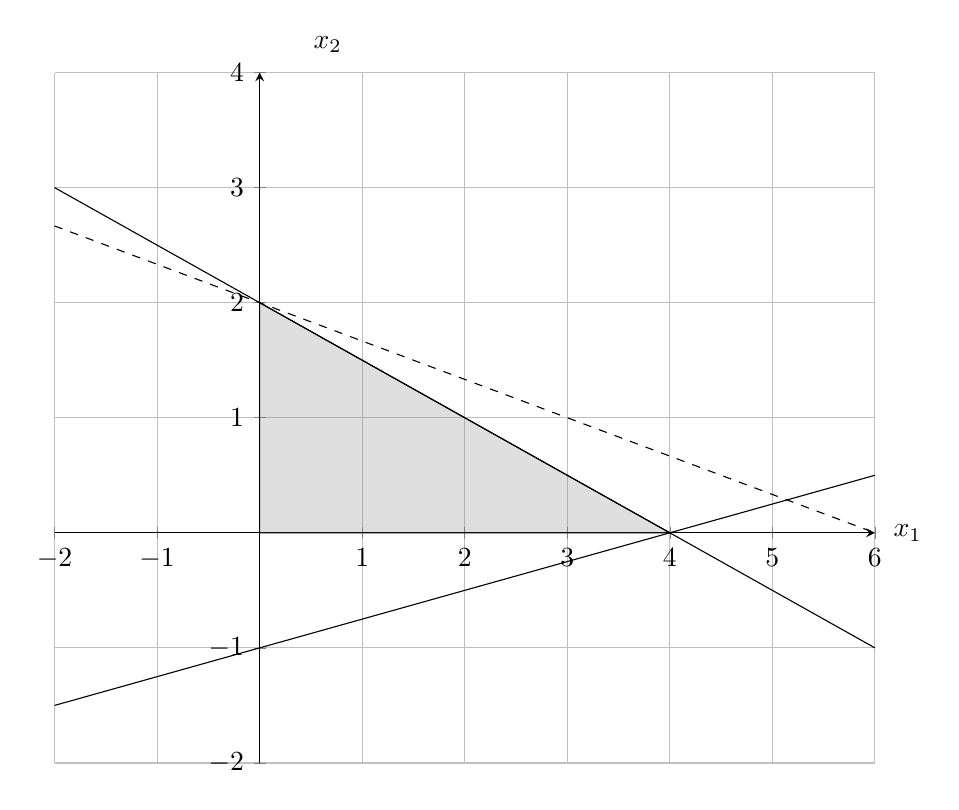
\begin{tikzpicture}
  \begin{axis}[ width=12cm, grid=both, axis x line=middle, axis y
    line=middle, title=, clip=false, ymin=-2, ymax=4, xmin=-2,
    xmax=6 ]

    \addplot[domain=-2:6] {-1 + 1/4*x}; \addplot[domain=-2:6] {2
      - 1/2*x}; \addplot[domain=-2:6,dashed] {2 - 1/3*x};
    \addplot[fill=gray, fill opacity=.25] coordinates { (0,0)
      (4,0) (0,2) }\closedcycle;

    % to get axis labels at the end of the axis
    \node at (axis description cs:1.04,.333) {$x_1$}; \node at
    (axis description cs:.333,1.04) {$x_2$};
  \end{axis}
\end{tikzpicture}
\end{center}

The feasible region for the linear program in part b) is unbounded;
however, since it is a minimization problem, it has an optimal
solution at $x_1=0$, $x_2=0$. The value of the objective function at
the optimal solution is $z=0$.

\begin{center}
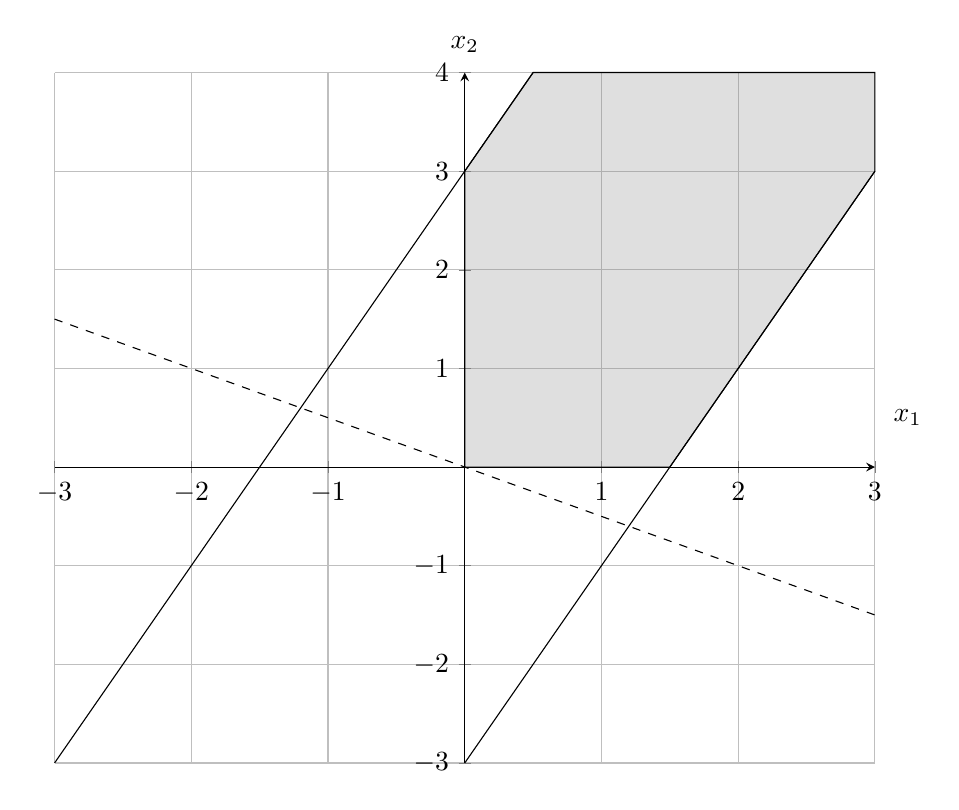
\begin{tikzpicture}
  \begin{axis}[ width=12cm, grid=both, axis x line=middle, axis y
    line=middle, title=, clip=false, ymin=-3, ymax=4, xmin=-3,
    xmax=3 ]

    \addplot[domain=0:3] {-3 +2*x}; \addplot[domain=-3:.5] {3+2*x};
    \addplot[domain=-3:3,dashed] {-1/2*x}; \addplot[fill=gray, fill
    opacity=.25] coordinates { (0,0) (0,3) (.5,4) (3,4) (3,3) (1.5,0)
    }\closedcycle;

    % to get axis labels at the end of the axis
    \node at (axis description cs:1.04,.5) {$x_1$}; \node at (axis
    description cs:.5,1.04) {$x_2$};
  \end{axis}
\end{tikzpicture}
\end{center}

\end{solution}

% re-written by Hannah
\item \emph{Karl's garden.}
Karl is a local gardener who grows lettuce, broccoli, and carrots. His garden is 
400 ft$^2$, and each individual plant of lettuce, broccoli, and carrots occupies 
0.5 ft$^2$, 1.2 ft$^2$, and 0.25 ft$^2$, respectively. Karl recently learned that 
many of his neighbors are interested in purchasing his vegetables. After polling the 
neighborhood, he learned that he has demand for 350 lettuce plants, 350 broccoli plants, 
and 250 carrot plants. Karl estimates that he will earn a profit of \$9.50 per 
lettuce plant, \$12.80 per broccoli plant, and \$8.25 per carrot plant. How many 
plants of each type of vegetable should Karl grow to maximize profit? Solve this 
problem using optimization software.

\begin{solution}
  \bs A GAMS model is provided in the file
  \texttt{karls-garden.gms}. The solution indicates that Karl should
  grow 350 lettuce plants, 135 broccoli plants, and 250 carrot plants
  for a total profit of about \$\num{7120}. Note that we are ignoring
  any fractional values of the decision variables.
\end{solution}


% this problem needs to be re-written, but I think we can just
% change the context and leave the numbers as they are (or very close
% anyway). the idea is to extract a shadow price and use it
% to answer questions.
\item \emph{Workplace safety.}  A manufacturing
  company has assembled a safety committee to reduce the number of
  injuries sustained by employees at work. The company has allotted
  the committee a budget of \$100 each week for purchasing items that
  will increase employee safety. After analyzing past incidents, the
  safety committee has concluded that the most common work hazard is
  exposure to loud noises. As a result, the committee would like to
  purchase (i) earplugs and (ii) other PPE (personal protection
  equipment). The relative value (utility) of the safety items was
  investigated, and it was determined that earplugs provide 1.2 units
  of value for each dollar spent on other types of PPE. The safety
  committee would like to determine how to spend the budget to
  maximize the safety of employees, but the company does not want to
  spend more than \$70 on earplugs and \$50 on other PPE each
  week. The committee also has the option to save part of the money.
  Additionally, the company would like to know:
\begin{enumerate}
\item How the total value of its expenditures for safety would change
  if there were only \$99 to spend. \label{safetya}
\item How the total value would change if \$75 could be spent on
  earplugs.\label{safetyb}
\item Whether it would save any money if each dollar of savings would
  provide 1.1 units of value for each dollar spent on other
  PPE.\label{safetyc}
\end{enumerate}
Formulate the safety committee's spending decision as a linear program. Sketch
the feasible region and determine the optimal solution using the
graphical method.  Then solve the linear program using optimization
software and obtain post-optimality output (i.e. a sensitivity
report).  Use this output to answer each of the questions \ref{safetya},
\ref{safetyb}, \ref{safetyc}.

\begin{solution}
\bs In the problem formulation to maximize total value, let
\[
  \begin{array}{lcl}
    x_1 &=& \textrm{\$ to spend on earplugs} \\
    x_2 &=& \textrm{\$ to spend on other PPE}
  \end{array}
\]
Then the committee wants to solve the following problem.
\[
\begin{array}{lrrrrr}
\textrm{maximize}   & 1.2x_1& +& x_2&      &   \\
\textrm{subject to} & x_1& +&x_2& \leq & 100 \\
                    & x_1& & & \leq & 70 \\
                    & & & x_2& \leq & 50 \\
\multicolumn{4}{r}{x_1,x_2}&       \geq & 0
\end{array}
\]

The feasible region is given below. The optimal solution is $x_1=70$ and $x_2=30$
for a total value of 114.
\begin{center}
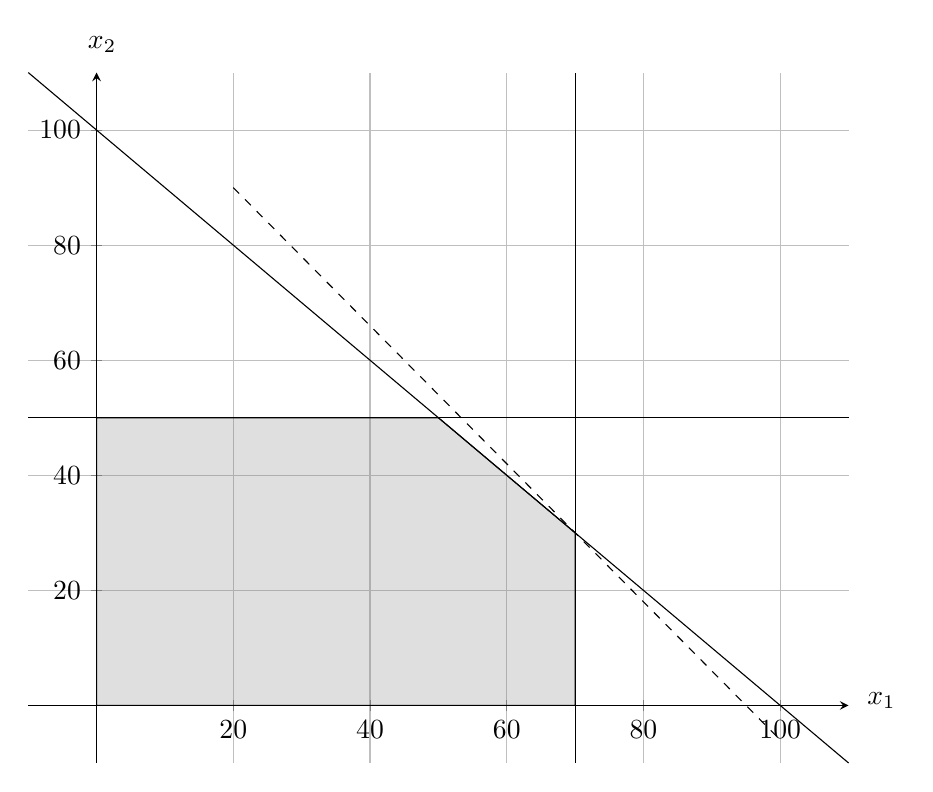
\begin{tikzpicture}
  \begin{axis}[ width=12cm, grid=both,
    axis x line=middle,
    axis y line=middle,
    title=, clip=false,
    ymin=-10, ymax=110, xmin=-10, xmax=110 ]

    \addplot[domain=-10:110] {-x + 100};
    \addplot[mark=none] coordinates {(70,-10) (70,110)};
    \addplot[domain=-10:110] {50};
    \addplot[fill=gray, fill opacity=.25] coordinates {
      (0,0) (70,0) (70,30) (50,50) (0,50) }\closedcycle;
    \addplot[domain=20:100,dashed] {-1.2*x + 114};

    % to get axis labels at the end of the axis
    \node at (axis description cs:1.04,.09) {$x_1$};
    \node at (axis description cs:.09,1.04) {$x_2$};
  \end{axis}
\end{tikzpicture}
\end{center}

A GAMS model is provided in \texttt{workplace-saftey.gms}. Refer to
the listing file \texttt{workplace-saftey.lst}, to answer questions
\ref{safetya}, \ref{safetyb}, and \ref{safetyc}.  Regarding part
\ref{safetya}, the shadow price on the \texttt{budget} constraint
tells us that if we decrease the RHS from 100 to 99, the value of the
objective function will decrease to 113. Since earplugs provide more
value than other PPE, the new solution will be $x_1=70$ and $x_2=29$.
For part \ref{safetyb}, notice that \$75 is within the range for the
shadow price on the \texttt{earplugs} constraint. So, increasing the
RHS to 75 will increase the total value by
\[ \$5 \times 0.2~\text{units of value per dollar} = 1 \]
for a total value of 115.
Finally, for part \ref{safetyc}, saving one dollar requires \$1; however, the
company gets 1.1 units of value for each dollar saved. Yes, the
company would save \emph{some} amount of money and spend less on other
PPE. To use the shadow price to answer this question, notice that the
shadow price on the \texttt{budget} constraint is 1. If we
``price-out'' the new activity of saving money, we see that it cost
\$1 per unit, but it returns \$1.1 per unit in total value. So the
company would save some amount of money. The question did not ask us
to determine the new solution. It only asked whether \emph{any} money
would be allocated to savings.
\end{solution}

% this problem needs to be re-written and GAMS code added.
\item \emph{A blending problem.}  A pet food manufacturer is
  developing a new dog food recipe with natural ingredients. It has
  been decided that the recipe will contain a combination of 4
  ingredients: chicken, brown rice, vegetables, and corn meal. The
  cost and important nutritional information for each ingredient is
  summarized in the table below.

\begin{center}
\begin{tabular}{lcccc} \\
Ingredient  &   Cost (\$/lb)  & Protein (g/lb)  &  Fat (g/lb) &  Fiber (g/lb)  \\ \hline
(1) Chicken   &  3.00 & 125 & 60 & 0 \\
(2) Brown rice   &  0.75 & 12 & 4 & 9 \\
(3) Vegetables   &  1.80 & 14 & 1.5 & 12 \\
(4) Corn meal& 0.60 & 32 & 8 & 17
\end{tabular}
\end{center}

Industrial engineers have been asked to determine the most
cost-effective mixture of ingredients given the following guidelines:
\begin{itemize}
\item Each pound of dog food must contain less than 40 grams of fat
\item Each pound of dog food must contain at least 80 grams of protein 
\item Each pound of dog food must contain between 4 and 10 grams of fiber
\item Each ingredient must comprise at least 10\% of the mixture
\end{itemize}

\begin{enumerate}
\item Formulate an (algebraic) mathematical programming model using
  the information above and generate a solution using software.
  \label{doga}

\item Formulate an alternative (algebraic) mathematical programming
  model given the additional constraint that 80\% of the mixture must
  contain a combination of chicken and vegetables. Generate a solution
  using software and determine the added cost due to the new
  constraint. \label{dogb}
\end{enumerate}

\begin{solution}
\bs For part \ref{doga}, a GAMS model is provided in the file \texttt{dog-fooda.gms}.
The mixture should contain 55.7\% chicken, 10\% brown rice, 10\% vegetables, and 24.3\% corn meal for a cost of \$2.07 per pound.
	
For part \ref{dogb}, A GAMS model is provided in
\texttt{dog-foodb.gms}. The added cost due to the additional
constraint is \$0.20. The mixture should contain 58\% chicken, 10\%
brown rice, 22\% vegetables, and 10\% corn meal for a cost of \$2.27
per pound.
\end{solution}


% re-written by Hannah
\item \emph{Golf lessons.}  Amy and Brian are professional
  golfers who have each agreed to donate 10 hours of private golf
  lessons to a charity auction. Three people have bid on the lessons,
  and their bids are shown in the table below. For example, Emma has
  bid \$28 per hour to receive lessons from Amy.

\begin{tabular}{lrr}
Bidder & Amy & Brian \\ \hline
Emma & \$28/hr & \$30/hr \\
Dan     & \$26/hr & \$28/hr \\
Sam  & \$30/hr & \$32/hr
\end{tabular}

In the spirit of fairness, the auction committee has decided that no bidder can win 
more than 8 hours of total instruction. Given the bid amounts, the committee must now
decide how to allocate the 20 hours of available instruction time.
\begin{compactenum}
  \item Draw a diagram of the problem as a network flow model.
  \item Formulate a linear programming model to maximize the
    charity's revenue.
  \item Solve the problem using optimization software.
\end{compactenum}

\begin{solution}
  \bs A diagram of the network flow model is shown below. Bidders 1, 2,
  and 3 correspond to Emma, Dan, and Sam, respectively.
\vspace{.2in}
\begin{center}
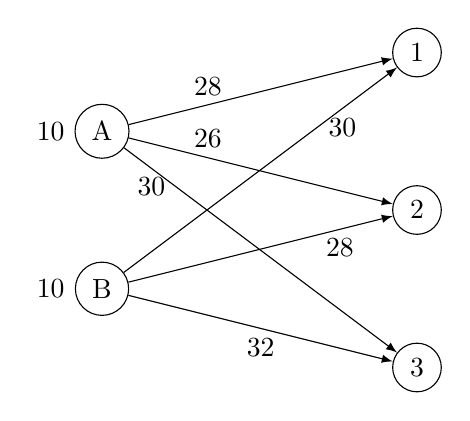
\begin{tikzpicture}[>=latex] % to get latex arrowheads

  \node[circle,draw](B) at (0,2) {B};
  \node[circle,draw](A) at (0,4) {A};
  \node[circle,draw](3) at (4,1) {3};
  \node[circle,draw](2) at (4,3) {2};
  \node[circle,draw](1) at (4,5) {1};

  \draw[->] (A) -- (1) node[above,pos=.3]{28};
  \draw[->] (A) -- (2) node[above,pos=.3]{26};
  \draw[->] (A) -- (3) node[below,pos=.1]{30};
  \draw[->] (B) -- (1) node[below,pos=.8]{30};
  \draw[->] (B) -- (2) node[below,pos=.8]{28};
  \draw[->] (B) -- (3) node[below,pos=.5]{32};

  \node[anchor=east] at (A) {10~~~~};
  \node[anchor=east] at (B) {10~~~~};

\end{tikzpicture}
\end{center}

Let $x_{ij}$ be the number of hours of instruction bidder $j$ receives
from professional golfer $i$.
  \[
     i \in \{\text{A},\text{B}\} \qquad j \in \{1,2,3\}
  \]
  The problem formulation is
\[
  \begin{array}{lrrrrrrrrrr}
    \textrm{maximize} &&&&&&&&&&\\   
    28x_{\text{A}1}&+& 26x_{\text{A}2}&+&30x_{\text{A}3}&+&30x_{\text{B}1}&+&28x_{\text{B}2}&+&32x_{\text{B}3} \\ \\
    \textrm{subject to}  &&&&&&&&&&\\
    & & & & x_{\text{A}1}&+ & x_{\text{A}2}&+ &x_{\text{A}3} & = & 10 \\
    & & & & x_{\text{B}1}&+ & x_{\text{B}2}&+ &x_{\text{B}3} & = & 10 \\
    & & & & & &  x_{\text{A}1} & + & x_{\text{B}1} & \leq & 8 \\
    & & & & & &  x_{\text{A}2} & + & x_{\text{B}2} & \leq & 8 \\
    & & & & & &  x_{\text{A}3} & + & x_{\text{B}3} & \leq & 8 \\
    \multicolumn{11}{r}{x_{ij} \geq 0 \quad \text{for}~i \in \{\text{A},\text{B}\},~j \in \{1,2,3\} }
  \end{array}
\]

The optimal solution is: bidder 1 (Emma) receives 6 hours of
instruction with Amy and 2 hours of instruction with Brian, bidder 2
(Dan) receives 4 hours of instruction with Amy, and bidder 3 (Sam)
receives 8 hours of instruction with Brian. The charity receives \$588
in revenue. A GAMS model and solution is provided in
\texttt{golf-lessons.gms}.  \emph{Note:} There are multiple optimal
solutions to this problem, so the values of the decision variables in
your solution could differ, but the value of the objective function
will be the same.
\end{solution}

% we need GAMS code for this problem, otherwise it's OK
\item \emph{A supply chain problem.} A company will produce the same
  new product at two different factories, and then the product will be
  shipped to two warehouses. Factory 1 can send an unlimited amount by
  rail to warehouse 1 only, whereas factory 2 can send an unlimited
  amount by rail to warehouse 2 only. However, independent truckers
  can can be used to ship up to 50 units from each factory to a
  distribution center (DC), from which up to 50 units can be shipped
  to each warehouse.  The shipping cost for each alternative is shown
  in the following table, along with the amounts to be produced and
  the amounts needed at the warehouses.

\begin{center}
\begin{tabular}{|l|r|r|r|r|}\hline
 & \multicolumn{3}{c|}{Unit shipping cost} & \\ \cline{2-4}
    & & \multicolumn{2}{c|}{Warehouse} & \\ \cline{3-4} 
\diagbox[width=10em]{From}{To}&  DC & WH1 & WH2 & supply \\ \hline
  Factory 1&  3 &  7 & -- & 80\\
  Factory 2&  4 &  --&  9 & 70\\
  DC       &    &  2 &  4 &   \\ \hline
  demand   &    & 60 & 90 &   \\ \hline
\end{tabular}
\end{center}

\begin{enumerate}
\item Draw the network representation of this problem as a transshipment problem.
\item Formulate the linear programming problem that minimizes total shipping cost.
\item Solve this problem using an algebraic modeling language such as GAMS.
\end{enumerate}

\begin{solution}
\bs

To make the notation easier, assign numbers to the nodes in the
network as follows: node 1 is factory 1, node 2 is factory 2, node 3
is the DC, node 4 is warehouse 1, and node 5 is warehouse 2.  Let
$x_{ij}$ be the number of products shipped from node $i$ to node $j$.

\begin{center}
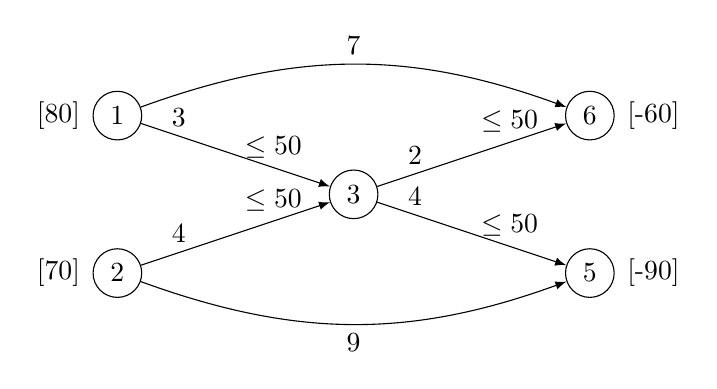
\begin{tikzpicture}[>=latex]
  \node[circle,draw](f1) at (0,2) {1};
  \node[circle,draw](f2) at (0,0) {2};
  \node[circle,draw](dc) at (3,1) {3};
  \node[circle,draw](wh2) at (6,0) {5};
  \node[circle,draw](wh1) at (6,2) {6};

  \node[anchor=east] at (f1) {[80]~~~~};
  \node[anchor=east] at (f2) {[70]~~~~};
  \node[anchor=west] at (wh1) {~~~[-60]};
  \node[anchor=west] at (wh2) {~~~[-90]};

  \draw[->] (f1) to [out=20,in=160]  node[above,pos=.5]{7} (wh1);
  \draw[->] (f2) to [out=340,in=200] node[below,pos=.5]{9} (wh2);
  \draw[->] (f1) -- (dc) node[above,pos=.2]{3} node[above,pos=.7]{$\leq 50$};
  \draw[->] (f2) -- (dc) node[above,pos=.2]{4} node[above,pos=.7]{$\leq 50$};
  \draw[->] (dc) -- (wh1) node[above,pos=.2]{2} node[above,pos=.7]{$\leq 50$};
  \draw[->] (dc) -- (wh2) node[above,pos=.2]{4} node[above,pos=.7]{$\leq 50$};
\end{tikzpicture}
\end{center}
  
\[
\begin{array}{lrrrrrrrrrrl}
\textrm{maximize} & 3x_{13} &+& 4x_{23} &+& 7x_{14} &+& 9x_{25} &+& 2x_{34} &+& 4x_{35} \\
  \textrm{subject to} &&&&&&& x_{12} &+& x_{14} &=& 80\\
                  &&&&&&& x_{23} &+& x_{25} &=& 70\\
                  &&&&&&& x_{34} &+& x_{14} &=& 60\\
                  &&&&&&& x_{25} &+& x_{35} &=& 90\\
  &&&&&&&&& x_{13} & \leq & 50\\
  &&&&&&&&& x_{23} & \leq & 50\\
  &&&&&&&&& x_{34} & \leq & 50\\
  &&&&&&&&& x_{35} & \leq & 50\\
  &&& x_{13} &+& x_{23} &-& x_{34} &-& x_{35} &=& 0\\
\multicolumn{10}{r}{x_{ij}} & \geq & 0
\end{array}
\]
The flow balance constraint at the DC is unnecessary because
total supply equals total demand. 
\end{solution}

\subsubsection*{Integer Programming}
% hannah
% the idea is that it is a set covering problem.
\item \emph{A set covering problem.}  A general merchandise retailer
  is planning to expand into a new metropolitan area comprised of
  seven cities. The following table shows the distance (in miles)
  between each city.

\begin{center}
\begin{tabular}{l|ccccccc}
& \multicolumn{7}{c}{To} \\
From & City 1 & City 2 & City 3 & City 4 & City 5 & City 6 & City 7\\ \hline
City 1 & 0 & 15 & 20 & 38 & 20 & 28 & 22 \\
City 2 & 15 & 0 &  5 & 23 & 16 & 12 & 10 \\
City 3 & 20 & 5 & 0 & 18 & 12 & 13 & 14 \\
City 4 & 38 & 23 & 18 & 0 & 31 & 19 & 27 \\
City 5 & 20 & 16 & 12 & 31 & 0 & 7 & 19 \\
City 6 & 28 & 12 & 13 & 19 & 7 & 0 & 22 \\
City 7 & 22 & 10 & 14 & 27 & 19 & 22 & 0 \\
\end{tabular}
\end{center}

The company assumes that customers will only visit a retail location
if it is within 15 miles of the city in which the customer
lives. Using this information, the company would like to construct the
fewest number of stores while ensuring that they can serve every
customer in the metropolitan area. Formulate an integer programming
model to determine the cities where retail locations should be
constructed.

\begin{solution}
\bs
\begin{equation*}
\text{Let $x_i$} = 
\begin{cases}
  1 & \text{if a retail location is constructed in city $i$,}\\
  0 & \text{otherwise.}
\end{cases}
\end{equation*}

To model the requirement that there is at least one retail location within
15 miles of city 1, we require that $x_1 + x_2 \geq 1$. The full
problem formulation is
\[
\begin{array}{lrrrrrrrrrrrrl}
\textrm{minimize} & \sum_{i=1}^{7} x_i & & & & & & \\
\textrm{subject to} && & & & & & & & x_1 & + & x_2 & \geq & 1 \\
& & & x_1 & + & x_2 & + & x_3 & + & x_6 & + & x_7 & \geq & 1 \\ & &  & x_2 & + & x_3 & + & x_5 & + & x_6 & + & x_7 & \geq & 1 \\
& &  & & & & & &  &  &  & x_4 & \geq & 1 \\
& & & &  & &  & x_3 & + & x_5 & + & x_6 & \geq & 1 \\
& & & &  & x_2 & + & x_3 & + & x_5 & + & x_6 & \geq & 1 \\
& & & & & & & x_2 & + & x_3 & + & x_7 & \geq & 1 \\
\multicolumn{14}{r}{x_i \in \{0,1\} \quad i = 1,\ldots,7}
\end{array}
\]
\end{solution}

% this problem needs to be re-written with a different context and
% different data.
\item \emph{A set partitioning problem.}  In a real estate development
  project, a residential area is divided into five tracts.  Two fire
  stations are to be constructed. There can be no more than one
  station in any tract. Furthermore, a station will respond to all
  fires in the tract in which it is located and to fires in the other
  tracts assigned to it.  The decisions to be made are
\begin{compactenum}
\item In which tracts are fire stations located
\item Assignment of the other tracts
\end{compactenum}
The objective is to minimize the overall average response time to fires.
Response times in the table below are in minutes.

\setlength{\tabcolsep}{7pt}
\renewcommand{\arraystretch}{1.2}
\newcolumntype{Y}{>{\centering\arraybackslash}X}
\begin{tabularx}{3.5in}{Y|rrrrrr}
  station located in tract  & \multicolumn{6}{l}{response time to fire in tract} \\
   & 1 & 2 & 3 & 4 & 5 &\\ \hline
  1 & 5 & 12 & 30 & 20 & 15 &\\
  2 & 20 & 4 & 15 & 10 & 25 &\\
  3 & 15 & 20 & 6 & 15 & 12 &\\
  4 & 25 & 15 & 25 & 4 & 10 &\\
  5 & 10 & 25 & 15 & 12 & 5 &\\ \hline
  average number of fires per day & 2 & 1 & 3 & 1 & 3 &
\end{tabularx}
\vspace{.2in}

Formulate a linear integer programming model that will locate the fire stations
and assign them to the other tracts without fire stations while minimizing
the overall average response time.
% need to put solution in LaTeX

% hannah
% integer programming with a fixed charge
\item \emph{A problem with a fixed charge.}  A bicycle manufacturing
  company can produce three types of bikes: mountain bikes, road
  bikes, and fat bikes. The company rents specific machinery for
  producing each type of bike. It costs \$150 per week to rent
  machinery for mountain bikes, \$250 per week to rent machinery for
  road bikes, and \$300 per week to rent machinery for fat bikes. A
  maximum of 120 hours of labor and \num{11000} pounds of material
  (aluminum) are available each week for production. The material
  and labor requirements to produce one unit of each type of bike are
  shown in the table below. The unit variable cost and the unit
  selling price for each type of bike are also shown.

\vspace{.1in}
\begin{tabulary}{5.4in}{LRRRR}
& Labor (hours) 
& Material (pounds) 
& Variable cost 
& Selling price \\ \hline
Mtn bike & 2.5 & 28 & \$350 & \$550 \\
Road bike & 7 & 25 & \$420 & \$800 \\
Fat bike & 4.5 & 36 & \$680 & \$\num{1200}
\end{tabulary}
\vspace{.1in}

The machinery needed to produce a specific type of bike is only rented
if that type of bike is produced. Assume that the company can sell all
of the bikes that it produces, regardless of type.  Formulate a mixed
integer linear programing problem to determine the weekly production
quantities of mountain bikes, road bikes, and fat bikes that will
maximize profit.

\begin{solution}
  \bs Let the decision variables $x_1,x_2,x_3$ be the number of
  mountain bikes, road bikes, and fat bikes, respectively, to produce
  each week. Machinery rental costs are only incurred if bicycles of that
  particular type are produced. We introduce binary decision variables
  $y_i$ to apply the machinery rental costs when production $x_i$ is
  positive.
\[
\text{Let $y_i$} = 
\begin{cases}
1 & \text{if $x_i > 0$} \\
0 & \text{otherwise}
\end{cases}
\quad i = 1,2,3.
\]
The mathematical formulation of the Integer Programming problem is
\[
\begin{array}{lrrrrrrl}
\textrm{maximize} &   & 550x_1 & + & 800x_2 & + & \num{1200}x_3 & \\
& - & 350x_1  & - & 420x_2 & - & 680x_3  & \\
& - & 150y_1& - & 250y_2&- & 300y_3& \\
& & & & & & &\\
\textrm{subject to} & 2.5x_1 & + & 7x_2 & + & 4.5x_3 & \leq & 120 \\
& 28x_1 & + & 25x_2 & + & 36x_3 & \leq & \num{11000} \\
& & & & & x_1 & \leq & My_1 \\
& & & & & x_2 & \leq & My_2 \\
& & & & & x_3 & \leq & My_3 \\
\end{array}
\]
where $M$ is a large number, $x_i \geq 0$, $x_i$ are integer-valued, 
$y_i \in \{0,1\}$, and $i = 1,2,3$.
\end{solution}

% this problem is OK.
\item \emph{Discrete purchases.} Sam is considering purchasing some
  combination of a new car, a washer, a dryer, and a high-definition
  television (HDTV). For practical reasons, Sam knows that he can only
  buy the dryer if he also buys the washer. It could still make sense
  to buy the washer without the dryer because Sam could dry his
  clothes on a clothesline. Due to political reasons with Sam's
  spouse, he can only purchase the HDTV if he does not purchase the
  car. Taking everything into consideration, Sam has estimated the
  values for each item. The item utilities (converted to dollars) and
  purchase prices in dollars are shown in the table below.  Sam's
  total budget is \$16,000. Formulate a binay integer programming
  problem to maximize Sam's estimated value while respecting the
  practicality, spouse, and budget constraints mentioned above.

\begin{center}
\begin{tabular}{lcc}
Item    &  Estimated value  & Price   \\  \hline
car     &   \$9,500   &  \$12,000 \\
washer  &   \$3,000   &  \$2,000  \\
dryer   &   \$3,000   &  \$2,000  \\
HDTV    &   \$5,000   &  \$3,000  \\
\end{tabular}
\end{center}

\begin{solution}
\bs

\[ \text{Let}~x_j = \begin{cases}
1 \quad \text{if item $j$ is purchased}\\
0 \quad \text{otherwise} \end{cases}
\]

where the index $j = 1,2,3,4$ corresponds to the car, washer, dryer,
and HDTV. The problem is to 
\[
\begin{array}{lrrrrrrrrl}
\textrm{maximize}   & 9.5x_1& +& 3x_2&+& 3x_3 &+& 5x_4 & & \\
  \textrm{subject to} & 12x_1& +& 2x_2&+& 2x_3 &+& 3x_4 & \leq & 16 \\
                    &&&&&& &x_3 & \leq & x_2 \\
  &&&&& x_1 & + & x_4 &\leq& 1 \\
\multicolumn{8}{r}{x_j}&  \in & \{0,1\}
\end{array}
\]
\end{solution}

% this problem needs to be re-written. the form of the problem should
% remain, but can we find a situation/problem to which this model
% would apply? we can change the coefficients if needed.
% no GAMS code is needed for this problem.
\item \emph{Modeling with binary variables.} Consider the problem:
\[
\begin{array}{lrrrrrrl}
\textrm{maximize} &   & z & = & x_1 & + & 2x_2 & \\
\textrm{subject to} & & & x_1 & + & x_2 & \leq & 8 \\
& & & -x_1 & + & x_2 & \leq & 2 \\
& & & x_1 & - & x_2 & \leq & 4 \\
& & & & & x_2 & \geq & \text{0, and integer} \\
& & & & & x_1 & = & \text{0,1,4, or 6} \\
\end{array}
\]

\begin{enumerate}
\item Reformulate the problem as an equivalent integer linear
  program.\label{ex:ip}
\item How would your answer to part \ref{ex:ip} change if the
  objective function were changed to:
\[ \text{maximize~} z = x_1^2 + 2x_2\text{?} \] \label{ex:quad}
\end{enumerate}

\begin{solution} 
\bs Introduce the following binary variables. Let
\[ y_i = \begin{cases}
    1 \quad \text{if}~ x_1 = i \quad i \in \{0,1,4,6\}\\
    0 \quad \text{otherwise}
    \end{cases}
  \]

Now the binary integer programming formulation is
\[
  \begin{array}{lrrrrrrrrl}
    \textrm{maximize}   &&& y_1 & + & 4y_4 & + & 6y_6 & + & 2x_2 \\
    \textrm{subject to} & y_0 & + & y_1 & + & y_4 & + & y_6 & = & 1 \\
                        & -y_1 & - & 4y_4 & - & 6y_6 & + & x_2 & \leq & 2\\
                        & y_1 & + & 4y_4 & + & 6y_6 & - & x_2 & \leq & 4\\
    \multicolumn{8}{r}{x_2}& \geq & 0 ~\text{and integer}\\
    \multicolumn{8}{r}{y_0,y_1,y_4,y_6}& \in & \{0,1\}
  \end{array}
\]
For part \ref{ex:quad}, change the coefficients on the $y_i$
variables in the objective function only to be the squares,
i.e. $16y_4$ and $36y_6$. Note that by using this technique the
objective function is transformed from a quadratic to a linear function
of the variables.
\end{solution}

\subsubsection*{Deterministic Dynamic Programming}

\subsubsection*{Deterministic Inventory Models}

% written by Emily
% deterministic inventory model
% to replace IMS problem 5 from ch 10
\item \emph{Ordering lumber.}  Building Builders, a construction
  company, always has a full schedule of building projects.  One of
  the most important resources required for their projects is
  lumber. To complete their projects, Building Builders has a constant
  demand for lumber of \num{5000} board feet per day.  There is a
  \$300\ delivery fee every time the company orders more lumber. It
  costs \$0.02\ per week for the company to store each unused board
  foot (7 days in one week). Every order has a lead time of 2 days to
  account for order processing and delivery time.

\begin{enumerate}
\item What is the optimal order quantity (in board feet) for Building
  Builders?
\item How frequently should Building Builders order to replenish the
  lumber supply?
\item Building Builders currently has space to store \num{35000} board
  feet of lumber. Should they invest in more space to store lumber?
  Why or why not?
\item What is the reorder point?
\end{enumerate}

\begin{solution}
  \bs The cost per order is $C_0=\$300$, the holding cost is
  $C_h=\$.02$ per board foot per week, the lead time is $m=2$ days,
  the demand rate is $D=\num{5000}$ board feet per day, and there are
  7 days in a week.  The demand per week is
  \[\num{5000} ~\text{board feet per day} \times 7 ~\text{days per
      week} = \num{35000} ~\text{board feet per week}\] Using the
  formula for economic order quantity,
\[ Q^{\ast} = \sqrt{\frac{2DC_o}{C_h}} = \sqrt{\frac{2(\num{35000})(300)}{0.02}} = \num{32404}~\text{board feet.} \]

The cycle time associated with the economic order quantity is
\[ T^{\ast} = \frac{Q^{\ast}}{D} = \frac{\num{32404}}{\num{5000}} = 6.5 ~\text{days.} \]

No, Building Builders should not invest in more space to store lumber
because the economic order quantity of \num{32404} board feet is less
than the current storage space capacity of \num{35000} board feet.

The lead time is 2 days and the usage rate per day is \num{5000} board
feet, so the reorder point is $2 \times \num{5000} = \num{10000}$
board feet.
\end{solution}


\end{enumerate}
